\chapter{The Search for Gravitational Waves}

\textcolor{blue}{Write 1-2 pages providing a synopis of the history of
GWs and programs to detect them.}

The field of ground-based gravitational-wave (GW) physics is rapidly
approaching a state with a high likelihood of detecting GWs for the
first time. Such a detection will not only validate part of Einstein's
general theory of relativity, but initiate an era of astrophysical
observation of the universe through GWs. Gravitational waves are
dynamic strains in space-time that travel at the speed of light and
are generated by non-axisymmetric acceleration of mass. The frequency
of the gravitational wave depends on its source. A first detection is
expected to witness an event such as a binary black hole/neutron star
merger. This chapter provides the theoretical framework of
gravitational wave generation and presents various ways to detect GWs,
including the current status of an effort to do so. I explain the
purpose of this dissertation in the context of these current effort,
and I conclude with an outline of the content found in the chapters
that follow.


\section{The Theory of Gravitational Radiation}
Gravitational radiation is a perturbation $|h_{\mu \nu}|
\ll 1$ to the flat space-time Minkowski metric $\eta_{\mu \nu} =
\mbox{diag}(-1, 1, 1, 1)$. The metric describing space-time in the
presence of gravitational radiation is therefore
\begin{equation}
g_{\mu\nu} = \eta_{\mu\nu} + h_{\mu\nu}.
\end{equation}
Just as in electrodynamics where one has freedom in choosing the
vector potential $\vec{A}$ for calculating the magnetic field $\vec{B}
= \vec{\nabla} \times \vec{A}$, one also has freedom in general
relativity in choosing the form of $h_{\mu \nu}$ for ease of calculation. A
convenient and popular choice is called the transverse-traceless (TT)
gauge in which
\begin{equation}
h_{\mu \nu} = 
\left\llbracket \begin{array}{c c c c} 
0 & 0 & 0 & 0\\ 
0 & h_+ & h_\times & 0 \\
0 & h_\times & -h_+ & 0 \\
0 & 0 & 0 & 0
\end{array} \right\rrbracket
\end{equation}
where the $+$ and $\times$ represent two linearly independent
polarizations. Without loss of generality, we consider the $h_+$
polarization in the example that follows.

For a gravitational wave traveling along the $z$ axis, the metric is
given by:
\begin{equation}
ds^2 = -c^2dt^2 + [1+h_+(t)] dx^2 + [1-h_+(t)] dy^2.
\end{equation}
This says the TT coordinate system is stretched along the $x$ axis and
and compressed along the $y$ axis by a factor of 
\begin{equation}
\sqrt{1 \pm h_+(t)} \approx 1 \pm \frac{1}{2} h_+(t).
\label{eq:deltaL}
\end{equation}
Therefore, the \emph{proper distance} between two free masses located
along either the $x$ or the $y$ axes changes by the factor in
Eq. \ref{eq:deltaL}; their coordinate separations remain constant. The
GW perturbation is a dimensionless strain
\begin{equation}
h = 2 \frac{\Delta L}{L}.
\end{equation}



\section{Sources}
Any object with an accelerating mass quadrupole moment generates
gravitational waves. The typical strain amplitudes, however, are
extremely tiny: a binary system of coalescing $1 \mbox{M}_\odot$
neutron stars in the Virgo Cluster (a distance of 15 Mpc) would
produce a maximum GW strain on Earth of only
$10^{-21}$. \textcolor{blue}{Not right--fix this!!} The strain is
proportional to source mass and velocity, and inversely proportional
to distance from the observer:
\begin{equation}
h \approx \frac{GMv^2}{Rc^4}
\end{equation}
Consequently, the most promising sources of detectable gravitational
waves are nearby, fast-moving, massive astrophysical objects that
include
\begin{itemize}
\item supernovae \vspace{-10pt}
\item binary stars (orbiting or coalescing) \vspace{-10pt}
\item spinning neutron stars \vspace{-10pt}
\item cosmological/astrophysical background
\end{itemize}
and can be categorized as producing periodic, burst, or stochastic GWs.

Stably orbiting binary star systems comprised of black holes or
neutron stars as well as rapidly spinning non-axisymmetric pulsars are
considered periodic sources since they will produce GWs
of relatively constant frequency. These reliable sources of GWs
require a long integration time to pick out their signal above
noise. The Hulse-Taylor binary, for instance, falls into this
category. Supernovae are burst sources since the gravitational
collapse will produce a short-lived, unmodeled emission of
GWs. Binaries in their final tens of milliseconds of inspiral also
fall into this category. Finally, the anisotropies in the inflation of
the universe together with the hum of all distant astrophysical
sources will create a stochastic background of radiation. Coherent
cross-correlation between multiple detectors is necessary for
measuring the constant amplitude, broad-spectrum GW background.

Directly detecting gravitational radiation from any such source will
reveal information that electromagnetic radiation cannot convey. The
frequency of the GW tells about the dynamical timescale of the
source. Only through GW radiation, for example, can mass and spin
properties of a black hole be revealed.





\section{Methods of Detection}
\begin{itemize}
\item Hulse/Taylor
\item Resonant bars
\item Pulsar timing
\item CMB polarization (B-modes)
\item Interferometry
\end{itemize}
For an approachable overview of the history of the field, including
detector design choices and estimated GW strain amplitudes of various
sources, refer to Ref. \cite{Linsay1983Study}.






\section{State of Ground-based Interferometry}
A network of first generation kilometer-scale laser interferometer
gravitational-wave detectors completed its integrated 2-year data
collection run in 2007, called S5. The instruments were: the American
Laser Interferometer Gravitational-wave Observatories (LIGO)\cite{Abbott2009LIGO},
one in Livingston, LA with 4 km long arms and two in Hanford, WA with
4~km and~2 km long arms; the 3~km French-Italian detector
VIRGO\cite{Acernese2008Virgo} in Cascina, Italy; and the 600~m
German-British detector GEO\cite{Luck2006Status} in Ruthe, Germany. Multiple
separated detectors increase detection confidence through signal
coincidence and improve source localization through triangulation.

The first generation of LIGO, known as Initial LIGO, achieved its
design goal of sensitivity to GWs in the 40~Hz - 7000~Hz band which
included a record strain sensitivity of
$2\times10^{-23}/\sqrt{\mathrm{Hz}}$ at 155~Hz. However, only the
loudest of sources produce enough GW strain to appear in LIGO's band,
and no gravitational wave has yet been found in the S5 data. A second
generation of LIGO detectors, Advanced LIGO, has been designed to be
at least an order of magnitude more sensitive at several hundred Hz
and above and include an impressive increase in bandwidth down to
10~Hz, dramatically increasing the chances of detection. The baseline
Advanced LIGO design \cite{AdvLigoSysDesign} improves upon Initial
LIGO by featuring better seismic isolation, the addition of a signal
recycling mirror at the output port, homodyne readout, and an increase
in laser power from 10~W to 165~W.

To test some of Advanced LIGO's new technologies so unforeseen
difficulties could be addressed and so that a more sensitive data
taking run could take place, increasing the chances of detection, an
incremental upgrade to the interferometers was carried out after S5
\cite{Adhikari2006Enhanced}. This project, Enhanced LIGO, culminated
with the S6 science run from July 2009 to October 2010.  An output
mode cleaner was designed, built and installed, and DC readout of the
GW signal was implemented \cite{Fricke2011DC}. An Advanced LIGO active
seismic isolation table was also built, installed, and tested
\cite[Ch. 5]{KisselThesis}. In addition, the 10~W Initial LIGO laser
was replaced with a 35~W laser
\cite{Frede2007Fundamental}. Accompanying the increase in laser power, 
the test mass Thermal Compensation System \cite{Willems2009Thermal},
the Alignment Sensing and Control, and the Input Optics were modified.

As of the writing of this dissertation (September 2011), construction
and installation of Advanced LIGO is underway. The vacuum systems are
being retro-fitted to accompany the new layout, and at LLO the 165~W
laser has been installed. At both sites, the new seismic isolation
platforms and multi-level suspension cages are being
mass-produced. The By 2012, the first of the suspended mirrors will be
installed and testing begun. Simultaneously, VIRGO and GEO are both
undergoing their own upgrades as well \cite{Acernese2008Virgo}
\cite{Luck2010Upgrade}. Figure \ref{fig:h_all} shows the achieved and
theoretical future noise curves of this network of ground-based GW
detectors.

\begin{figure}
\begin{centering}
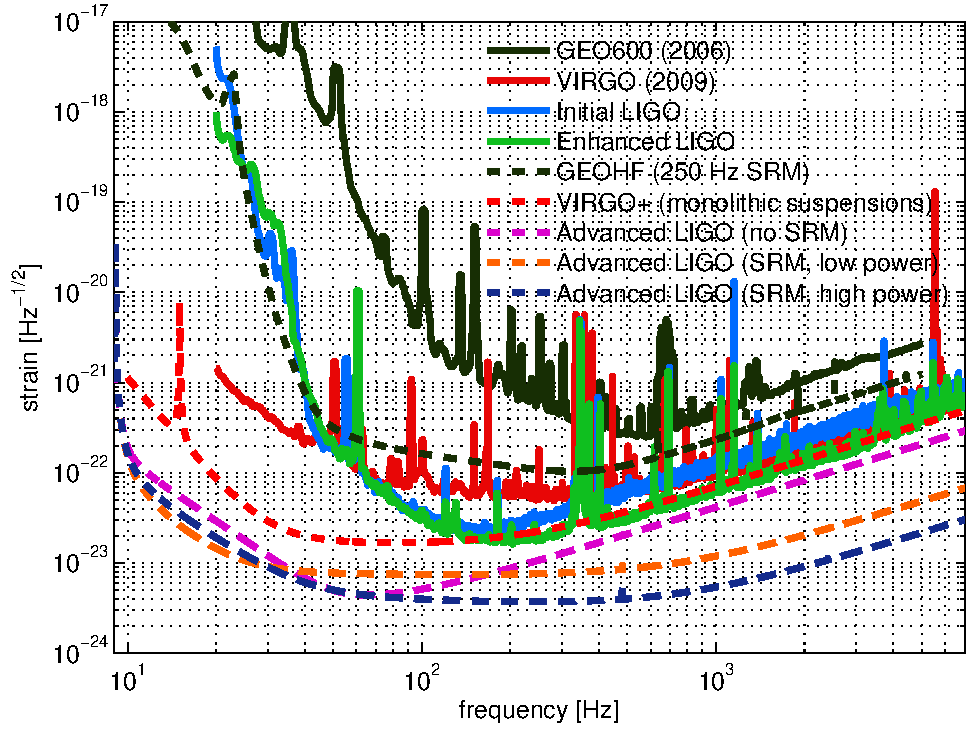
\includegraphics[width=1.0\textwidth]{figures/GWnetwork_strains.pdf}
\caption[Strain sensitivities of LIGO-VIRGO collaboration interferometers]{Strain sensitivities of LIGO-VIRGO collaboration interferometers.}
\label{fig:h_all}
\end{centering}
\end{figure}


\section{Purpose of this Work}
The purpose of this work is to demonstrate the capability of an
interferometric gravitational wave detector to operate at several
times the highest of laser powers previously used. From a na\"ive
standpoint, more power is desirable since strain sensitivity improves
by $\sqrt{P}$ in the high frequency ($>$ 200~Hz) shot-noise-limited
region. However, as detectors become more sensitive at low frequencies
($<$ 70 Hz) in the years to come, radiation pressure noise will become
the dominant noise source there, making high laser power operation a
design trade-off. Currently, seismic noise limits low frequency
sensitivity, so exploring the technical world of increasing the laser
power is a fruitful adventure.

%Although offering an improvement to the shot-noise-limited sensitivity, 
More power introduces radiation pressure and thermally induced side
effects that must all be addressed for effective interferometer
operation. Concerns about the practical difficulties of handling high
power effects abounded during Initial LIGO when operating at the
design power of 10~W proved more difficult and less straight-forward
than expected. To achieve the Advanced LIGO design sensitivity, an
ambitious 160~W of input power is needed. Without an understanding of
the thermal and radiation pressure problems at 10~W, Advanced LIGO
becomes a daunting goal.

The work presented in this dissertation was carried out during
Enhanced LIGO to verify and investigate the predicted and unforeseen
effects of as much as 25~W of laser power. I present the design and
the measurements I made of the performance of two of the
interferometer subsystems that are affected by an increase in laser
power: the Input Optics and the Angular Sensing and Control. I show
that the thermal and radiation pressure effects on these subsystems
are well understood and should not pose \textcolor{blue}{unsolvable,
  pick different word} problems for
Advanced LIGO.
% As an
% epilogue, I make projections of what can be expected for Advanced LIGO
% based on the results of my experimental studies. 


\subsection{The Input Optics High Power Story} 
The performance of the Initial LIGO Input Optics degraded as the
result of absorbing too much heat while the input power ramped up to
7~W. Particular issues that needed to be addressed for any further
increase in power included thermal steering of the beam rejected by
the interferometer, a decrease in the optical isolation, and thermal
lensing that drove the spatial mode of the beam directed at the
interferometer away from optimal. I describe the design of the
improved Input Optics for Enhanced LIGO which includes less absorptive
optical components in order to conquer thermal issues at the source
and changes to the design architecture that compensate for any
residual effects. I also present the set of measurements I made to
characterize the Input Optics performance with up to 30~W input
power. I show that we can expect the Input Optics to perform well for
Advanced LIGO.



\subsection{The Angular Sensing and Control High Power Story}
Radiation pressure creates torques, a long-known concept, and the
optical torque's ability to de-stabilize optical cavities was first
recognized in 1991 by Solimeno et
al. \cite{Solimeno1991FabryPerot}. However, the theory of radiation
pressure's effect on angular mechanical transfer functions was not
fully appreciated and published until 2006 by Sidles and Sigg
\cite{Sidles2006Optical}. The concern arised that radiation pressure
might be the factor limiting Initial LIGO's ability to increase the
input power. Eiichi Hirose showed that the optical torque was present
and measurable, but that it was \emph{not} limiting Initial LIGO's
power \cite{Hirose2010Angular}.\footnote{In fact, after the Enhanced
  LIGO laser was installed, and before any changes were made to the
  ASC, we successfully operated the interferometer with 14~W input
  power.} % Nov. 20, 2008 elog.
The concern of the optical torque's role in cavity dynamics shifted to
Enhanced and Advanced LIGO, which were designed to operate at four
times and 20 times the laser power of Initial LIGO, respectively. Lisa
Barsotti developed a numerical model of the angular sensing and
controls for Enhanced LIGO, specifically including radiation pressure
torque. She showed that, in principle, the radiation pressure torque
can be controlled without detrimental consequences to the sensitivity
of the detector \cite{Barsotti2009Modeling}. We implemented Barsotti's
theoretical control scheme and I measured its performance with up to
20~W of input power, demonstrating a thorough understanding of the
principles at work and providing confidence in the ability to control
radiation pressure torques in Advanced LIGO. I also improved upon
Hirose's measurement of the optical angular (anti-)spring. In
addition, through post-analysis of angular data, I demonstrate the
potential of a technique that may be used in Advanced LIGO for
reducing the angular control signals.



\subsection{Outline of this Dissertation}
The organization of this dissertation is as follows. Chapter~2
describes the measurement apparatus, the LIGO interferometer, focusing
on key aspects which are relevant for the rest of the thesis,
including the motivation for more laser power. Chapter~3 presents the
design and performance of the Enhanced LIGO Input Optics with up to
30~W input power. Chapter~4 introduces the Angular Sensing and
Control, describing the causes of angular mirror motion, why angular
motion matters, and how it was sensed and controlled in Initial
LIGO. Chapter~5 derives the coupled cavity eigenfunctions that result
from radiation pressure torque, setting the stage for changes to the
ASC to accompany high power. Chapter~6 presents the characterization
and performance of the Enhanced LIGO ASC with up to 20~W input power,
and Chapter~7 shows the direct measurement of the optical
(anti-)spring. A summary and conclusions are in Chapter~8.

